\documentclass{article}
\usepackage[letterpaper, total={6.5in, 9in}]{geometry}
\usepackage{graphicx} % Required for inserting images
\usepackage{hyperref}
\usepackage[simplified]{pgf-umlcd}
\usepackage{pdflscape}
\usepackage{xcolor}

\renewcommand {\umltextcolor}{black}
\renewcommand {\umlfillcolor}{white}
\renewcommand {\umldrawcolor}{black}

% \usepackage{emoji}  % LuaLaTeX
% \setemojifont{TwemojiMozilla}

\title{Processing Relay Chat -- PRC}
\author{David Chen -- Team PLA (Pretty Lazy Acronym)}
\date{Period 6}

\begin{document}

\maketitle

\section{Description}
Processing Relay Chat (PRC) encompasses a client program, server program, and protocol for instant messaging over the network. To accomplish this in Processing PRC the \href{https://processing.org/reference/libraries/net/index.html}{Network} library.\\
PRC will include the following features:
\begin{itemize}
    \item Ephemeral plaintext (printable ASCII)\footnote{Due to font limitations, Unicode glyphs for other languages/emojis cannot be fully supported.} messaging
    \item Usernames with deterministic colors
    \item A slash command framework for advanced user interaction
    \item Image embedding, including animated GIFs
    \item Chat log export
\end{itemize}

\subsection{Protocol}
PRC uses a JSON-like TCP packet schema, in which ASCII separator characters are used, simplifying the burden of packet parsing. Commands include:
\begin{itemize}
   \item SEND packets to send user messages
   \item NAME packets to set user nickname
   \item JOIN packets to create/join channels
   \item CHAN packets listing the available channels
\end{itemize}

%\begin{landscape}
\section{UML Diagram}
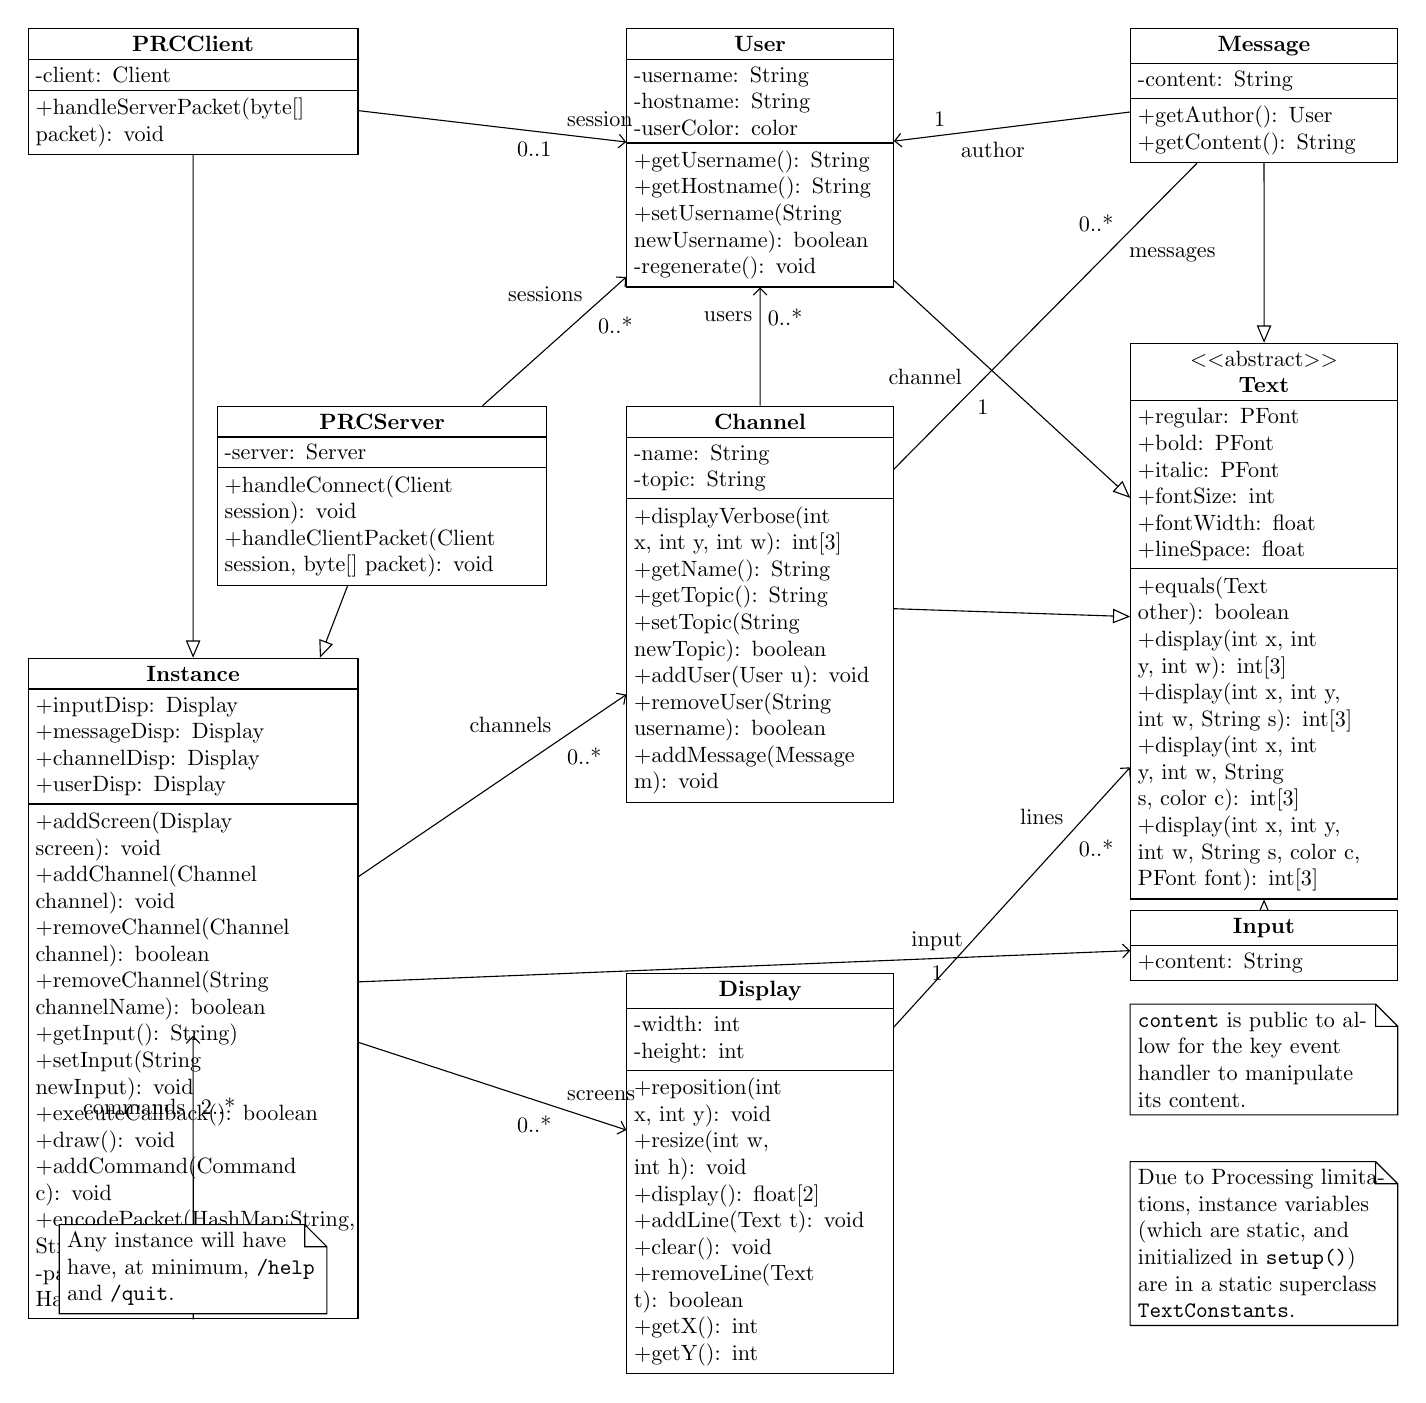
\begin{tikzpicture}
\begin{scope}[scale=0.8, transform shape]
    \begin{abstractclass}[text width = 4cm]{Text}{20,3}
        \attribute{+regular: PFont}
        \attribute{+bold: PFont}
        \attribute{+italic: PFont}
        \attribute{+fontSize: int}
        \attribute{+fontWidth: float}
        \attribute{+lineSpace: float}
        \operation{+equals(Text other): boolean}
        \operation{+display(int x, int y, int w): int[3]}
        \operation{+display(int x, int y, int w, String s): int[3]}
        \operation{+display(int x, int y, int w, String s, color c): int[3]}
        \operation{+display(int x, int y, int w, String s, color c, PFont font): int[3]}
    \end{abstractclass}
        \umlnote[draw] at (20, -10) (text) {Due to Processing limitations, instance variables (which are static, and initialized in \verb|setup()|) are in a static superclass \verb|TextConstants|.};

    \begin{class}[text width = 4cm]{Display}{12,-7}
        \attribute{-width: int}
        \attribute{-height: int}
        \operation{+reposition(int x, int y): void}
        \operation{+resize(int w, int h): void}
        \operation{+display(): float[2]}
        \operation{+addLine(Text t): void}
        \operation{+clear(): void}
        \operation{+removeLine(Text t): boolean}
        \operation{+getX(): int}
        \operation{+getY(): int}
    \end{class}
    \unidirectionalAssociation{Display}{lines}{0..*}{Text}

    \begin{class}[text width = 4cm]{Input}{20, -6}
        \inherit{Text}
        \attribute{+content: String}
    \end{class}
    \umlnote[draw] at (20, -7.5) (input-note) {\verb|content| is public to allow for the key event handler to manipulate its content.};

    \begin{class}[text width = 4cm]{User}{12, 8}
        \inherit{Text}
        \attribute{-username: String}
        \attribute{-hostname: String}
        \attribute{-userColor: color}
        \operation{+getUsername(): String}
        \operation{+getHostname(): String}
        \operation{+setUsername(String newUsername): boolean}
        \operation{-regenerate(): void}
    \end{class}

    \begin{class}[text width = 4cm]{Channel}{12,2}
        \inherit{Text}
        \attribute{-name: String}
        \attribute{-topic: String}
        \operation{+displayVerbose(int x, int y, int w): int[3]}
        \operation{+getName(): String}
        \operation{+getTopic(): String}
        \operation{+setTopic(String newTopic): boolean}
        \operation{+addUser(User u): void}
        \operation{+removeUser(String username): boolean}
        \operation{+addMessage(Message m): void}
    \end{class}
    \unidirectionalAssociation{Channel}{users}{0..*}{User}

    \begin{class}[text width = 4cm]{Message}{20, 8}
        \inherit{Text}
        \attribute{-content: String}
        \operation{+getAuthor(): User}
        \operation{+getContent(): String}
    \end{class}
    \association{Channel}{channel}{1}{Message}{0..*}{messages}
    \unidirectionalAssociation{Message}{author}{1}{User}

    \begin{abstractclass}{Command}{3,-8}
        \operation{+getName(): String}
        \operation{+getHelp(): String}
        \operation{+execute(String[] args): void}
    \end{abstractclass}

    \begin{class}[text width = 5cm]{Instance}{3,-2}
        \attribute{+inputDisp: Display}
        \attribute{+messageDisp: Display}
        \attribute{+channelDisp: Display}
        \attribute{+userDisp: Display}
        \operation{+addScreen(Display screen): void}
        \operation{+addChannel(Channel channel): void}
        \operation{+removeChannel(Channel channel): boolean}
        \operation{+removeChannel(String channelName): boolean}
        \operation{+getInput(): String)}
        \operation{+setInput(String newInput): void}
        \operation{+executeCallback(): boolean}
        \operation{+draw(): void}
        \operation{+addCommand(Command c): void}
        \operation{+encodePacket(HashMap<String, String> src): String}
        \operation{-parsePacket(byte[] packet): HashMap<String, String>}
    \end{class}
    \begin{class}{PRCServer}{6, 2}
        \inherit{Instance}
        \attribute{-server: Server}
        \operation{+handleConnect(Client session): void}  % serverEvent()
        \operation{+handleClientPacket(Client session, byte[] packet): void}  % Server.available() - server receives packet
    \end{class}
    \begin{class}{PRCClient}{3, 8}
        \inherit{Instance}
        \attribute{-client: Client}
        \operation{+handleServerPacket(byte[] packet): void}  % clientEvent() - client receives packet
    \end{class}
    \unidirectionalAssociation{Instance}{screens}{0..*}{Display}
    \unidirectionalAssociation{Instance}{channels}{0..*}{Channel}
    \unidirectionalAssociation{Instance}{commands}{2..*}{Command}
    \unidirectionalAssociation{Instance}{input}{1}{Input}
    \unidirectionalAssociation{PRCClient}{session}{0..1}{User}
    \unidirectionalAssociation{PRCServer}{sessions}{0..*}{User}

    \umlnote[draw] at (3, -11) (commands-note) {Any instance will have have, at minimum, \verb|/help| and \verb|/quit|.};
\end{scope}
\end{tikzpicture}
%\end{landscape}
\newpage

\section{Manual}
The main Processing program will serve as a launcher, allowing the user to select from server or client modes.

\subsection{Server Mode}
The user will be able to select a TCP port for the server to broadcast on.

The program will then display a log of server interactions (user connections, messages, disconnections). The user can quit the program using \verb|/quit|.

\subsection{Client Mode}
The user will then enter a server address/port to connect to. On successful connection, the user can register a username, which the server will check for uniqueness. If the username is rejected, the user is prompted to enter another username.

The client will then be offered a list of channel names (and their corresponding topics). The client can choose to connect to a channel, upon which they will be put into a chat window view.


\subsubsection{Chat Window}
The main chat window will display messages, usernames, and timestamps. Below the chat window, an input will be available for user messages/commands.

\paragraph{Slash Commands}
To join a room, use \verb|/join|. To leave a room, use \verb|/leave.| To quit the client, use \verb|/quit| (aliased to \verb|/q|).

For information on further commands, use \verb|/help|.

\section{Functionality}
The goal for the coming week is to begin the initial framework for PRC; implementing all minimum features described in the specification.

\subsection{Issues}
\begin{enumerate}
    \item To share font data among \verb|Text| subclasses, it was appropriate to use \verb|static| variables, but there may be "non-\verb|static| inner type" issues when trying to declare \verb|static| variables in the \verb|Text| abstract class. To fix this, the abstract class itself must be declared \verb|static|. (\href{https://forum.processing.org/two/discussion/23623/when-creating-a-class-what-is-it-an-inner-class-of-declared-static-in-a-non-static-inner-type.html}{Source})
    \item In testing, it appears that a Client and a Server running in the same PApplet may lead to unexpected behavior. Thus, it will be necessary to run the server separately from the client.
\end{enumerate}

\section{Log}
\begin{itemize}
    \item 05/20: Began writing program specifications in \LaTeX.
    \item 05/21 -- 05/22: Constructed UML class diagrams for anticipated object classes.
    \item 05/23 -- 05/24: Corrected text location alignment issues.
    \item 05/25: Implemented Text subclasses and display() functions; turned Text into an abstract base class to deduplicate logic; Implemented Display and constructed a testing mockup.
    \item 05/26 -- 05/28: Adjusted UML class designs to provide additional necessary functionality. Began working on network transmission of messages.
    \item 05/29 -- 06/02: Worked around rendering bug that prevented messages from instantly appearing on the screen. Began pondering design and protocol alterations for separate Client/Server classes, along with proper maintainance of message, channel, and user states.
\end{itemize}

\end{document}
